\documentclass[conference]{IEEEtran}
\pdfsuppressptexinfo=-1
\pdfinfoomitdate=1
\pdftrailerid{}
\usepackage[utf8]{inputenc}
\usepackage[T1]{fontenc}
\usepackage{graphicx}
\usepackage{booktabs}
\usepackage{url}
\usepackage{cite}
\usepackage{amsmath}
\usepackage{xcolor}
\begin{document}
\pdfinfo{/Author (Huda Mueen)}

\title{Post Quantum Session Authentication for Drone Command Links: Executed Baselines, Flight Stack in the Loop and Replay Rules}
\author{\IEEEauthorblockN{Huda Mueen}\IEEEauthorblockA{Independent researcher, United Arab Emirates\\hudamueen2407@gmail.com}}
\maketitle

\begin{abstract}
Flight controllers fielded today may still be in service when an attacker can forge classical signatures and break classical key exchange. We execute six command channel designs on the same cores and fly five of them with the same flight stack and link: MAVLink 2 signing as shipped, a classical session (X25519, Ed25519), a post quantum only session (ML-KEM-768, ML-DSA-44), a hybrid session of both, a session authenticated only by pinned static ML-KEM-768 keys, and an ML-DSA-44 signature on every command. On two open RISC-V core designs in cycle accurate RTL simulation, the hybrid session costs 1.75 to 1.89 times the vehicle side computation of the classical session, the KEM authenticated session 1.03 to 1.13 times, and a signature per command 292 to 371 times a per message tag. With ArduPilot in the loop over an emulated telemetry radio and real cryptography, the hybrid session keeps the share of commands acknowledged within 0.5~s, outages included, at 0.931 against 0.935 without authentication, while a signature per command drops it to 0.418, a figure that moves to 0.851 at a 1~s deadline. A strict next counter rule loses \mbox{0.033} of the acknowledged share on paired seeds, mostly through resynchronisations after outages; a replay cache loses nothing against the published rule. ProVerif proves injective agreement on commands for a cache that never forgets and checks and records each counter in one step, and for a window of two counters under the same assumption, and finds that the KEM authenticated session loses key secrecy once ML-KEM alone is broken. The code, data, logs and scripts are public at \url{https://github.com/hudasol/post-quantum-security}.
\end{abstract}

\section{Introduction}
A small multirotor runs its flight stack on a microcontroller and receives commands over a telemetry radio of tens of kilobits per second. MAVLink 2, the common protocol, offers a per message tag with a pre shared key \cite{mavsign}; without it, commands can be injected from the radio side \cite{kwon18,koubaa19}, and key establishment and endpoint authentication are left to the operator. A pre shared key is not broken by a quantum computer, but one stolen key exposes every past and future session that used it, and a fleet must provision and rotate such keys by hand; our model of a provisioned key with fresh nonces finds no forward secrecy for that reason. A session key exchange removes both problems, and its public key part is what a quantum computer threatens. Vehicles and their firmware stay in service for years, so a key exchange or signature that a future quantum computer breaks would let an attacker inject commands in real time during that service life. The replacements are standardised: ML-KEM for key establishment \cite{fips203} and ML-DSA for signatures \cite{fips204}.

Hyoung et al.\ measure post quantum TLS handshakes over an emulated drone radio and argue that, after the handshake, commands should carry only a symmetric tag \cite{hyoung26}; the per command cost there is derived, not measured, and acceptance of reordered or lost commands is not considered. Primitive benchmarks \cite{pqm4}, post quantum TLS on embedded systems \cite{burstinghaus20,gonzalez22} and KEM based authentication \cite{kemtls20,kemtlspdk21,pqwg21,pqnoise22} answer other parts. What an engineer cannot yet read from published evidence is how complete command channel designs, including a signature free KEM authenticated one, compare on the same core, the same link and the same flight stack, and what the replay rule does to availability.

This paper contributes:
(1) executed baselines of six command channel designs on two open RISC-V core designs in cycle accurate RTL simulation, with correctness checks, intervals over 15 runs, stack and code size, under one compiler and pinned libraries (Section~\ref{sec:rtl});
(2) ArduPilot in the loop with gateways that execute the real handshakes, tags and replay rules on paired seeds, with the sensitivity of each result to the command deadline (Section~\ref{sec:sitl});
(3) ProVerif models of the hybrid and the KEM authenticated sessions and of replay rules that accept out of order delivery, with the bounds of each model (Section~\ref{sec:formal});
(4) a pre registered, script checked method in which every number in this paper is read from a committed result file.

\section{Threat model and designs}
\label{sec:design}
\emph{Threat model.} The attacker controls the radio: it reads, drops, delays, reorders and injects frames and replays old ones, and it may hold a quantum computer during the service life of the vehicle. Endpoints, their long term keys and the flight stack are trusted; side channels, jamming beyond the modelled loss and outages, and the confidentiality of commands are out of scope. The goals are mutual authentication of the session endpoints, secrecy of the session key that keys the tags, and injective agreement on commands: every accepted command was sent by the ground station in that session and is accepted at most once.

\emph{Session designs.} All sessions end with the MAVLink 2 signing field of 13~B per message, keyed by the session key \cite{mavsign}. \emph{Classical}: X25519 key exchange, Ed25519 signatures by both sides over the transcript and both identities, key confirmation tags. \emph{Post quantum only}: ML-KEM-768 and ML-DSA-44 in the same roles. \emph{Hybrid} (proposed): X25519 and ML-KEM-768 together, the session key derived from both secrets and a transcript hash, ML-DSA-44 signatures by both sides; a design in which only the ground station signs leaves the vehicle unauthenticated in our model, and the vehicle signature (fix F1, not to be confused with flight F1) closes it. \emph{KEM authenticated} (design K): each side holds the other's static ML-KEM-768 key; the ground station sends an X25519 share, an ephemeral ML-KEM-768 key and an encapsulation to the vehicle's static key, the vehicle answers with its share, a ciphertext to the ephemeral key, an encapsulation to the ground station's static key and a confirmation tag, and the ground station confirms; there are no signatures, as in post quantum WireGuard and KEMTLS with pre distributed keys \cite{pqwg21,kemtlspdk21}. Table~\ref{tab:flights} gives the bytes of each flight.

\emph{Baselines without a session.} \emph{Signing as shipped}: a provisioned key, no handshake. \emph{Signature per command}: an ML-DSA-44 signature on every command, verified by the vehicle; like the corresponding baseline of the mission model below it carries no counter, so it does not resist replay and is weaker than the sessions.

\emph{Replay rules.} The vehicle accepts a command under one of three rules: \emph{published} (counter greater than the last accepted, gaps allowed) \cite{mavsign}; \emph{strict} (only the next counter; the ground station starts a new handshake when its link layer gives up a frame, or when the vehicle asks because a later counter arrived and the next did not); and \emph{replay cache} (any counter not yet accepted within a window of 64 counters).

\begin{table}[t]
\centering
\caption{Bytes per handshake flight as built by the executed protocols}
\label{tab:flights}
\setlength{\tabcolsep}{3pt}
\begin{tabular}{lrrrrr}
\toprule
Design & F1 & F2 & F3 & F4 & Total \\
\midrule
Classical & 32 & 32 & 80 & 80 & 224 \\
PQ only & 1,184 & 1,088 & 2,436 & 2,436 & 7,144 \\
Hybrid, F1 & 1,216 & 1,120 & 2,436 & 2,436 & 7,208 \\
KEM auth. (K) & 2,304 & 2,224 & 16 & -- & 4,544 \\
\bottomrule
\end{tabular}

\smallskip\footnotesize F1 and F3 ground to vehicle, F2 and F4 vehicle to ground; MAVLink framing and link fragmentation not included.
\end{table}

\section{Method}
\label{sec:method}
\emph{RTL simulation.} Ibex in its small configuration \cite{ibex} and CV32E40P \cite{cv32e40p}, both RV32IMC without caches or wait states, are simulated cycle accurately with Verilator. One firmware image per design runs the vehicle and the ground side, each step timed with the cycle counter, 15 runs per session image with a fixed seed block (5 for the deterministic tag image); every run checks that both sides derive the same key, that all signatures and tags verify, and known answers for the hash functions. Medians carry 95\% intervals over runs. Libraries are pinned and unmodified: mlkem-native \cite{mlkemnative}, mldsa-native \cite{mldsanative} and Monocypher \cite{monocypher}, all portable C, compiled with one compiler at \texttt{-O3}. Peak stack is measured by stack painting and includes the harness; code size is the text section of each image with unused sections removed, both sides and the harness included.

\emph{Software in the loop.} ArduPilot Copter 4.7.2 \cite{ardupilot} flies a scripted mission of about 48~s (take off, two legs, land) with its built in vehicle model; the ground station sends one acknowledged command per second. A relay emulates a SiK class radio of 64~kbit/s with independent frame loss of 0.02, link layer retransmission that can deliver frames out of order, and one outage per mission starting 15--40~s after arming with an exponential duration of mean 5~s; an outage longer than 10~s tears the session down. A gateway pair in front of the ground station and the flight stack executes the handshake, the tags and the replay rule with the same algorithms (Python cryptography and host builds of the same libraries). Vehicle side operations are released after a delay equal to their Ibex cycles at 168~MHz, fixed from the first runs before the flights (for design K, flown later, from the medians of all runs); ground side compute runs at host speed. The configurations fly 20 missions each on the same seeds, so they see the same outages and command phases. Acknowledged shares carry bootstrap intervals over missions, and differences between configurations are paired by mission; the number of commands per configuration ranges from 958 to 972. The host was slower than the applied delay for 2,695 of 212,157 vehicle side tags (at most 1,178 in one configuration) and 173 tag checks; these are counted, not corrected. For comparison, a mission model of the same traffic with independent loss and Poisson outages (60 per hour, about one per mission) gives availability per rule; its strict rule adds a stall per resynchronisation but neither the airtime of the new handshake nor rejections of reordered frames.

\emph{Formal models.} ProVerif \cite{proverif} checks secrecy, agreement and reachability under a Dolev Yao attacker with abstract primitives and unbounded sessions. Session models carry one command, a rekey and a further command per session; replay cache models carry three commands per key; the bounded window is modelled on the command layer for a window of two counters. Rekey grace periods, counter wrap and timestamps are not modelled. Breaking a component is modelled by giving its secrets to the attacker.

\emph{Discipline.} 14 predictions with refutation clauses were hashed before the runs and scored by script under the less favourable reading of any ambiguous clause: 12 hit, 1 between and 1 missed. The thresholds were broad, so the hits say less than the misses, and design K was added after registration. Every number in this paper is registered with its file, column and query and checked by a script in continuous integration.

\section{Executed baselines on core designs}
\label{sec:rtl}
\begin{table}[t]
\centering
\caption{Executed baselines: million cycles per unit (RTL simulated, medians of 15 runs) and code size on CV32E40P (host measured)}
\label{tab:rtl}
\setlength{\tabcolsep}{2.5pt}
\begin{tabular}{lrrrrr}
\toprule
 & \multicolumn{2}{c}{Vehicle} & \multicolumn{2}{c}{Ground} & Code \\
Design & Ibex & CV32E40P & Ibex & CV32E40P & (kB) \\
\midrule
MAVLink 2 tag$^{a}$ & 0.015 & 0.013 & 0.014 & 0.013 & 21.7 \\
Classical session & 15.5 & 12.4 & 15.4 & 12.4 & 44.9 \\
PQ only session & 23.8 & 17.3 & 21.6 & 15.4 & 56.1 \\
Hybrid session, F1 & 29.2 & 21.8 & 32.3 & 23.9 & 66.5 \\
KEM auth.\ session (K) & 17.4 & 12.8 & 20.2 & 14.7 & 46.0 \\
ML-DSA-44 per command$^{b}$ & 5.4 & 3.9 & 10.0 & 7.4 & 37.8 \\
\bottomrule
\end{tabular}

\smallskip\footnotesize Session rows: one session start. $^{a}$ check (vehicle) and generation (ground) of one tag over a COMMAND\_LONG frame. $^{b}$ verification (vehicle) and signing (ground) of one command.
\end{table}

\begin{figure}[t]
\centering
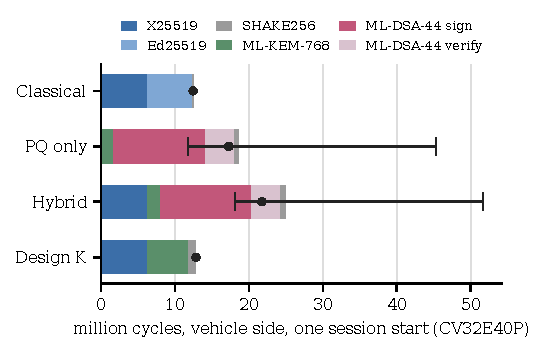
\includegraphics[width=\columnwidth]{fig_rtl.pdf}
\caption{Vehicle side cycles of one session start on CV32E40P by primitive (RTL simulated, medians). Bars are sums of primitive medians; the whisker is a bound, the bar total if its one signature took the fastest or the slowest ML-DSA-44 signing observed; the dot is the measured session median.}
\label{fig:rtl}
\end{figure}
Table~\ref{tab:rtl} gives the cost of one session start and of one command. The hybrid session costs 1.75$\times$ [1.59, 1.77] the classical vehicle side on CV32E40P and 1.89$\times$ [1.72, 1.91] on Ibex; on the ground side, which signs first, 1.92$\times$ and 2.09$\times$. Over the post quantum only session it costs 1.26$\times$ [1.05, 1.41] on the vehicle side and 1.55$\times$ on the ground side. The two designs differ by two X25519 multiplications, a fixed cost, while ML-DSA-44 signing repeats with rejection and took 5.6 to 39.2~M cycles per signature (Fig.~\ref{fig:rtl}); the spread of a signing design comes from there. With Monocypher, one X25519 multiplication (3.16~M cycles on CV32E40P) costs more than an ML-KEM-768 encapsulation (1.70~M), and an Ed25519 verification 4.53~M; this is a property of one portable C library designed for size, and a faster classical library would raise every ratio over the classical session.

Design K avoids both ML-DSA-44 operations: its vehicle side costs 1.03$\times$ the classical session and 0.59$\times$ [0.55, 0.65] the hybrid one, it needs 18.8~kB of stack against 50.5~kB for the hybrid (2.1~kB classical), and it carries 4,544~B in three flights against 7,208~B for the hybrid session, which is 32$\times$ the classical handshake. Code, counted for both sides and the harness together, grows from 44.9~kB (classical) to 66.5~kB (hybrid) and 46.0~kB (design K). After the handshake a command costs a tag check of 13,314 cycles on a COMMAND\_LONG (the tag alone, without parsing); verifying an ML-DSA-44 signature on the same frame instead costs 292$\times$ as much, and signing it on the ground side about twice that. At 168~MHz the vehicle side of the hybrid session start would take about 130~ms on CV32E40P (estimated), against 74~ms for the classical session. Ibex needs 1.34$\times$ the cycles of CV32E40P for the same hybrid handshake, so a cycle count for one core of an instruction set does not transfer to another.

\section{Flight stack in the loop and availability}
\label{sec:sitl}
\begin{table*}[t]
\centering
\caption{ArduPilot in the loop over an emulated SiK class radio, 20 paired missions per configuration}
\label{tab:sitl}
\setlength{\tabcolsep}{3pt}
\begin{tabular}{lrrr}
\toprule
Configuration & Handshake (s) & Added round trip (ms) & Share acknowledged within 0.5~s [95\% CI] \\
\midrule
No authentication & -- & ref. & 0.935 [0.902, 0.963] \\
MAVLink 2 signing as shipped$^{a}$ & -- & 4.0 & 0.932 [0.902, 0.962] \\
Classical session & 0.19 & 4.3 & 0.935 [0.904, 0.965] \\
Hybrid, published rule & 1.49 & 4.4 & 0.931 [0.896, 0.961] \\
Hybrid, strict rule & 1.50 & 4.3 & 0.898 [0.858, 0.936] \\
Hybrid, replay cache & 1.44 & 4.2 & 0.932 [0.899, 0.964] \\
Design K, published rule & 0.92 & 4.7 & 0.934 [0.903, 0.964] \\
ML-DSA-44 per command & -- & 496.1 & 0.418 [0.374, 0.459] \\
\bottomrule
\end{tabular}

\smallskip\footnotesize Handshake: median from F1 until both sides hold the key (vehicle accepting F3 for design K, ground accepting F4 otherwise), emulated link and executed cryptography with RTL derived vehicle delays. Added round trip: median round trip to the flight stack's acknowledgement against no authentication (SITL measured). Acknowledged share includes one outage per mission. $^{a}$ signing inside ArduPilot and the ground station at host speed, without RTL derived delays.
\end{table*}
\begin{figure}[t]
\centering
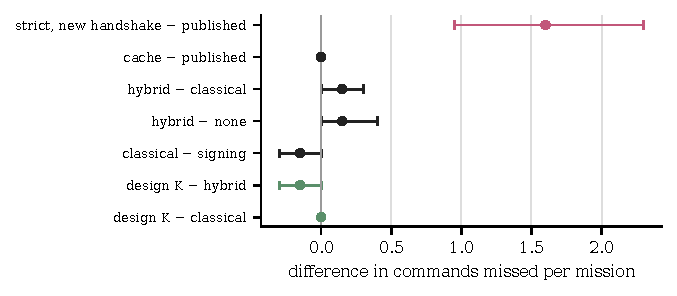
\includegraphics[width=\columnwidth]{fig_sitl.pdf}
\caption{Left: paired differences of the share acknowledged within 0.5~s with 95\% intervals over missions (SITL measured). Right: share acknowledged against the deadline (SITL measured, the same runs).}
\label{fig:sitl}
\end{figure}
Table~\ref{tab:sitl} and Fig.~\ref{fig:sitl} show that once a session exists, its per message cost is that of the shipped tag: the hybrid session adds 4.4~ms to the median command round trip, the classical session 4.3~ms and signing as shipped 4.0~ms, the last inside the flight stack and the ground station at host speed. These few milliseconds are mostly the gateway hops: the applied tag delays are 0.08 to 0.13~ms. The hybrid handshake takes 1.49~s over the emulated radio against 0.19~s for the classical session, a cost paid once per session. Design K completes its handshake in 0.92~s and differs from the hybrid session by \mbox{+0.0033} (\mbox{+0.0003} to \mbox{+0.0067}) and from the classical session by \mbox{-0.0007} (\mbox{-0.0014} to \mbox{-0.0002}); it was flown after the other configurations, alone on the host, on the same seeds, and the host overran the applied tag delay most often in its runs (1,178 tags), so this comparison is less clean than the others. The paired differences resolve a small cost of the hybrid session: \mbox{-0.0041} (\mbox{-0.0090} to \mbox{-0.0006}) against no authentication and \mbox{-0.0040} (\mbox{-0.0082} to \mbox{-0.0007}) against the classical session.

A signature on every command adds 496.1~ms to each round trip, mostly airtime of the 2.4~kB signature, since the applied verification delay is 32~ms; this puts the median round trip next to the deadline: 0.418 of its commands are acknowledged within 0.5~s, 0.636 within 0.55~s, 0.743 within 0.75~s and 0.851 within 1~s, against a drop of \mbox{0.51} from the hybrid session at 0.5~s. The mission model gives 0.730 at 0.5~s; we have not resolved this difference and report only the measured value.

The replay rule matters as much as the algorithms once a session exists. Link layer retransmission delivers some frames after newer ones (reordering depth up to 2), and the published rule rejected 11 of them as late. The strict rule, which here resynchronises by a full new handshake, loses \mbox{0.033} of the acknowledged share against the published rule (paired 95\% CI \mbox{0.019} to \mbox{0.047}). Its cost comes mainly from resynchronisation, not from reordering: 58 commands were lost while no session existed during 12 resynchronisations, 10 of them triggered when the link layer gave up a frame during an outage, against 13 rejected as ahead of the expected counter. The replay cache accepted the reordered frames that the published rule rejected: its difference to the published rule is \mbox{+0.0006} (\mbox{+0.0002} to \mbox{+0.0013}), a small gain. The mission model puts the strict rule cost at -0.0092, outside the paired interval; it underestimates the cost because it omits the airtime of the new handshake and the rejections.

\section{Formal results}
\label{sec:formal}
ProVerif checked 140 queries in 33 model files: 97 proved, 39 counterexamples and 3 that the tool could not prove, and 1 reached the time limit. Of the counterexamples, 12 are reachability checks that must fail (they show that the vehicle can accept a command, so agreement is not proved vacuously); the others are found in the designs before the fixes, including fallback and firmware update models not discussed here, in deliberate controls with a broken component or a missing check, and in the two results below that matter for the designs. With F1 the hybrid session keys stay secret and each side authenticates the other; the keys stay secret when either the classical or the KEM component is broken, and after a later theft of the long term keys.

Design K keeps its keys secret when the classical component is broken and after a later theft of the static keys, and the vehicle authenticates the ground station. With ML-KEM broken, however, its keys are not secret: the attacker sends its own first flight with stolen static keys, and the X25519 share does not save the session against an active attacker, whereas the hybrid session still has its signatures. Authentication of the vehicle by the ground station is proved only in a model in which static and ephemeral KEM keys have distinct types; the general model reached the time limit of 1800~s without a result.

For out of order delivery, a replay cache proves injective agreement on commands when the vehicle checks and records each pair of session and counter in one step and never forgets an entry, a condition stated in the model as a restriction, not derived. When concurrent branches read a table before either records, the model gives a counterexample, and a table read in sequence could not be proved; an implementation must therefore check and record atomically. The cache in the flights uses a bounded window, which was proved only on the command layer for a window of two counters, and the published timestamp rule could not be proved.

\section{Discussion and limitations}
For streamed commands the results support a session: its post quantum cost is paid once, and the per command cost stays that of the shipped tag. Where both identities can be pinned, design K needs 0.59 of the vehicle side cycles and about a third of the stack of the hybrid session, at the price of resting authentication on ML-KEM alone; the hybrid session keeps the classical component as a guard against a flaw in ML-KEM, while its authentication rests on ML-DSA-44 alone; a break of ML-DSA was not modelled. A signature per command fits rare, high value commands with a deadline of about a second, not a stream. The replay rule should be a replay cache that checks and records atomically.

\emph{Threats to validity.} (i) Cycles come from two open core designs with single cycle memories, applied in the loop at a Cortex-M4 clock; Cortex-M flight controllers have flash wait states, caches and other multipliers, and an earlier run of portable C code on Ibex took 2.2 to 2.9 times the published portable C cycles on Cortex-M4 and 3.5 to 4.3 times its assembly for ML-KEM-768 and ML-DSA-44 verification and key generation, and stack optimised signing \cite{greconici21} or RISC-V extensions \cite{alkim20,fritzmann20} would change the figures. (ii) One classical library was measured, and it favours the post quantum designs. (iii) In the loop, vehicle compute is a delay at an assumed clock, applied per event without a busy processor, so frames arriving during a verification are not queued behind it; the host was slower than the delay for a small share of tags. (iv) The radio is an emulation with independent frame loss and one scripted outage per mission; real loss is bursty. (v) Twenty missions per configuration, a bootstrap over missions that may under cover, and no correction for the several paired comparisons. (vi) Prior work figures are not comparable to ours because platforms and links differ; Table~\ref{tab:rw} compares methods, not figures. The next step is to repeat the executed baselines on Cortex-M4 and Cortex-M33 boards and to fly design K over a real telemetry radio.

\section{Related work}
Primitives are benchmarked on Cortex-M4 with pqm4 \cite{pqm4}, with stack optimised Dilithium \cite{greconici21} and with RISC-V extensions \cite{alkim20,fritzmann20}. Post quantum TLS has been measured on embedded clients \cite{burstinghaus20} and under loss \cite{paquin20,sikeridis20}; KEMTLS \cite{kemtls20,gonzalez22,kemtlspdk21}, post quantum WireGuard and Noise \cite{pqwg21,pqnoise22} authenticate by encapsulation. Firmware signatures have been measured on low power boards and in secure boot \cite{banegas21,kumar20,wagner22,campos20}. For drones, MAVSec encrypts MAVLink \cite{mavsec19}, Ahmed et al.\ combine two ML-KEM-768 encapsulations with ML-DSA-65 certificates and compute radio times without a flight stack \cite{ahmed26}, and de Meneses et al.\ verify a post quantum EDHOC variant with estimated costs \cite{meneses26}; for vehicle to vehicle messages, frame loss can decide practicality \cite{twardokus24}. Table~\ref{tab:rw} compares the closest works with this paper.

\begin{table*}[t]
\centering
\caption{Closest prior work and this paper (as recorded from each source)}
\label{tab:rw}
\setlength{\tabcolsep}{2pt}
\footnotesize
\begin{tabular}{llllll}
\toprule
Work & Platform & Link and stack & Per command cost & Availability & Formal check \\
\midrule
\cite{hyoung26} & x86 laptop & emulated UAV radio, TLS 1.3 & derived, not measured & not reported & none reported \\
\cite{burstinghaus20} & Cortex-A53, ESP32, others & Ethernet or Wi-Fi, network excluded & not reported & not reported & none reported \\
\cite{kemtls20,kemtlspdk21} & server or host & emulated network, TLS variants & not reported & not reported & proof on paper \\
\cite{pqwg21} & virtual machines & virtual network, WireGuard & not reported & not reported & Tamarin, with replay \\
\cite{ahmed26} & x86 laptop & none; SiK radio times computed & not reported & not reported & proof on paper \\
\cite{meneses26} & modelled Cortex-M4 & UAV, EDHOC variant, computed delays & not reported & not reported & Tamarin \\
\cite{twardokus24} & V2V chipset & DSRC, simulated and on road & measured & frame loss ratio & proof on paper \\
This paper & two RISC-V cores (RTL) & emulated SiK radio, ArduPilot & executed (RTL) & measured per rule & ProVerif \\
\bottomrule
\end{tabular}
\end{table*}

\section{Conclusion}
Executed under one set of conditions, a hybrid post quantum session for drone commands costs 1.75 to 1.89 times the vehicle side computation of a classical session on these cores (medians; more on the ground side and in expectation, because signing repeats) and many times its handshake bytes, yet leaves the per command cost and the availability of the shipped tag almost unchanged, while a signature per command does not at a 0.5~s deadline. A KEM authenticated session with pinned keys is the cheapest post quantum option but rests on ML-KEM alone. The replay rule decides as much as the algorithms: a strict rule that resynchronises by a new handshake loses commands after outages, while a replay cache loses nothing against the published rule; its proof covers a cache that checks and records in one step.

\bibliographystyle{IEEEtran}
\bibliography{references}
\end{document}
